%
% $RCSfile: design.tex,v $
%
% Copyright (C) 2002-2008. Christian Heller.
%
% Permission is granted to copy, distribute and/or modify this document
% under the terms of the GNU Free Documentation License, Version 1.1 or
% any later version published by the Free Software Foundation; with no
% Invariant Sections, with no Front-Cover Texts and with no Back-Cover
% Texts. A copy of the license is included in the section entitled
% "GNU Free Documentation License".
%
% http://www.cybop.net
% - Cybernetics Oriented Programming -
%
% http://www.resmedicinae.org
% - Information in Medicine -
%
% Version: $Revision: 1.1 $ $Date: 2008-08-19 20:41:06 $ $Author: christian $
% Authors: Christian Heller <christian.heller@tuxtax.de>
%

\subsection{Design}
\label{design_heading}
\index{Design Pattern}

Gamma et al. \cite{gamma1995} define a design pattern as: \textit{description of
collaborating objects and classes which are taylored to solve a general design
problem in a special context.} Mostly, patterns are in relation to each other.
They can be combined to master more complex tasks.

%
% $RCSfile: command.tex,v $
%
% Copyright (c) 2004. Christian Heller. All rights reserved.
%
% No copying, altering, distribution or any other actions concerning this
% document, except after explicit permission by the author!
% At some later point in time, this document is planned to be put under
% the GNU FDL license. For now, _everything_ is _restricted_ by the author.
%
% http://www.cybop.net
% - Cybernetics Oriented Programming -
%
% http://www.resmedicinae.org
% - Information in Medicine -
%
% @author Christian Heller <christian.heller@tuxtax.de>
%

\paragraph{Command}
\label{command_heading}

The \emph{Command} pattern \cite{gamma1995}, also known as \emph{Action} or
\emph{Transaction}, sometimes also \emph{Signal}, encapsulates a command in
form of an object. That way, operations can get parameterised; they can be put
in a queue, be made undone or traced in a log book. Figure \ref{command_figure}
shows the structure of the pattern.

\begin{figure}[ht]
    \begin{center}
        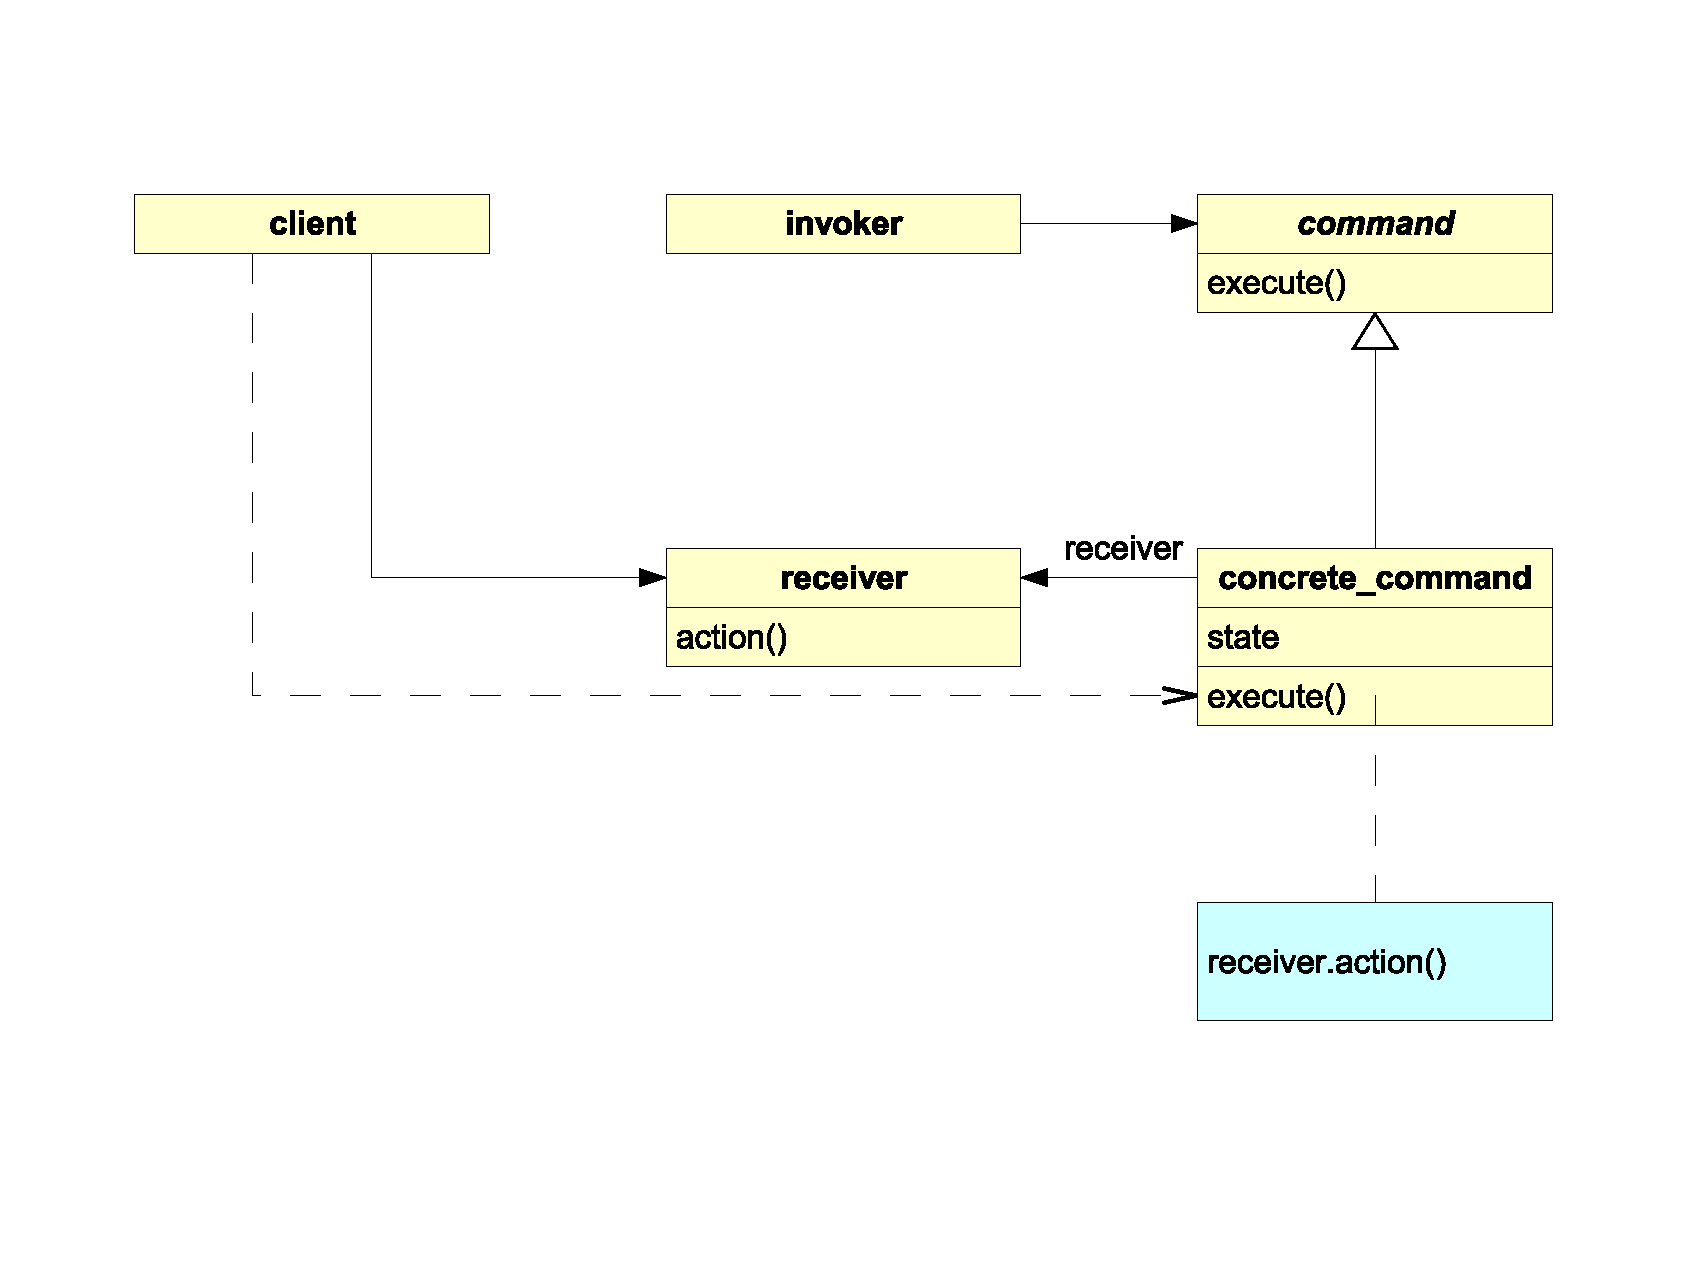
\includegraphics[scale=0.3]{vector/command.eps}
        \caption{Command Pattern}
        \label{command_figure}
    \end{center}
\end{figure}

%
% $RCSfile: wrapper.tex,v $
%
% Copyright (C) 2002-2008. Christian Heller.
%
% Permission is granted to copy, distribute and/or modify this document
% under the terms of the GNU Free Documentation License, Version 1.1 or
% any later version published by the Free Software Foundation; with no
% Invariant Sections, with no Front-Cover Texts and with no Back-Cover
% Texts. A copy of the license is included in the section entitled
% "GNU Free Documentation License".
%
% http://www.cybop.net
% - Cybernetics Oriented Programming -
%
% http://www.resmedicinae.org
% - Information in Medicine -
%
% Version: $Revision: 1.1 $ $Date: 2008-08-19 20:41:09 $ $Author: christian $
% Authors: Christian Heller <christian.heller@tuxtax.de>
%

\subsubsection{Wrapper}
\label{wrapper_heading}
\index{Wrapper Pattern}
\index{Adapter Pattern}
\index{Delegation Pattern}

The \emph{Wrapper} pattern \cite{gamma1995} allows otherwise incompatible
classes to work together. It can be seen as skin object enclosing (wrapping) an
inner core object, to which it provides access. In other words: It adapts the
interface of a class which is why Gamma et al. call the pattern \emph{Adapter}.
As can be seen in figure \ref{wrapper_figure}, this pattern makes heavy use of
\emph{Delegation}, where the \emph{Delegator} is the adapter (or wrapper) and
the \emph{Delegatee} is the class being adapted \cite{portland}.

\begin{figure}[ht]
    \begin{center}
        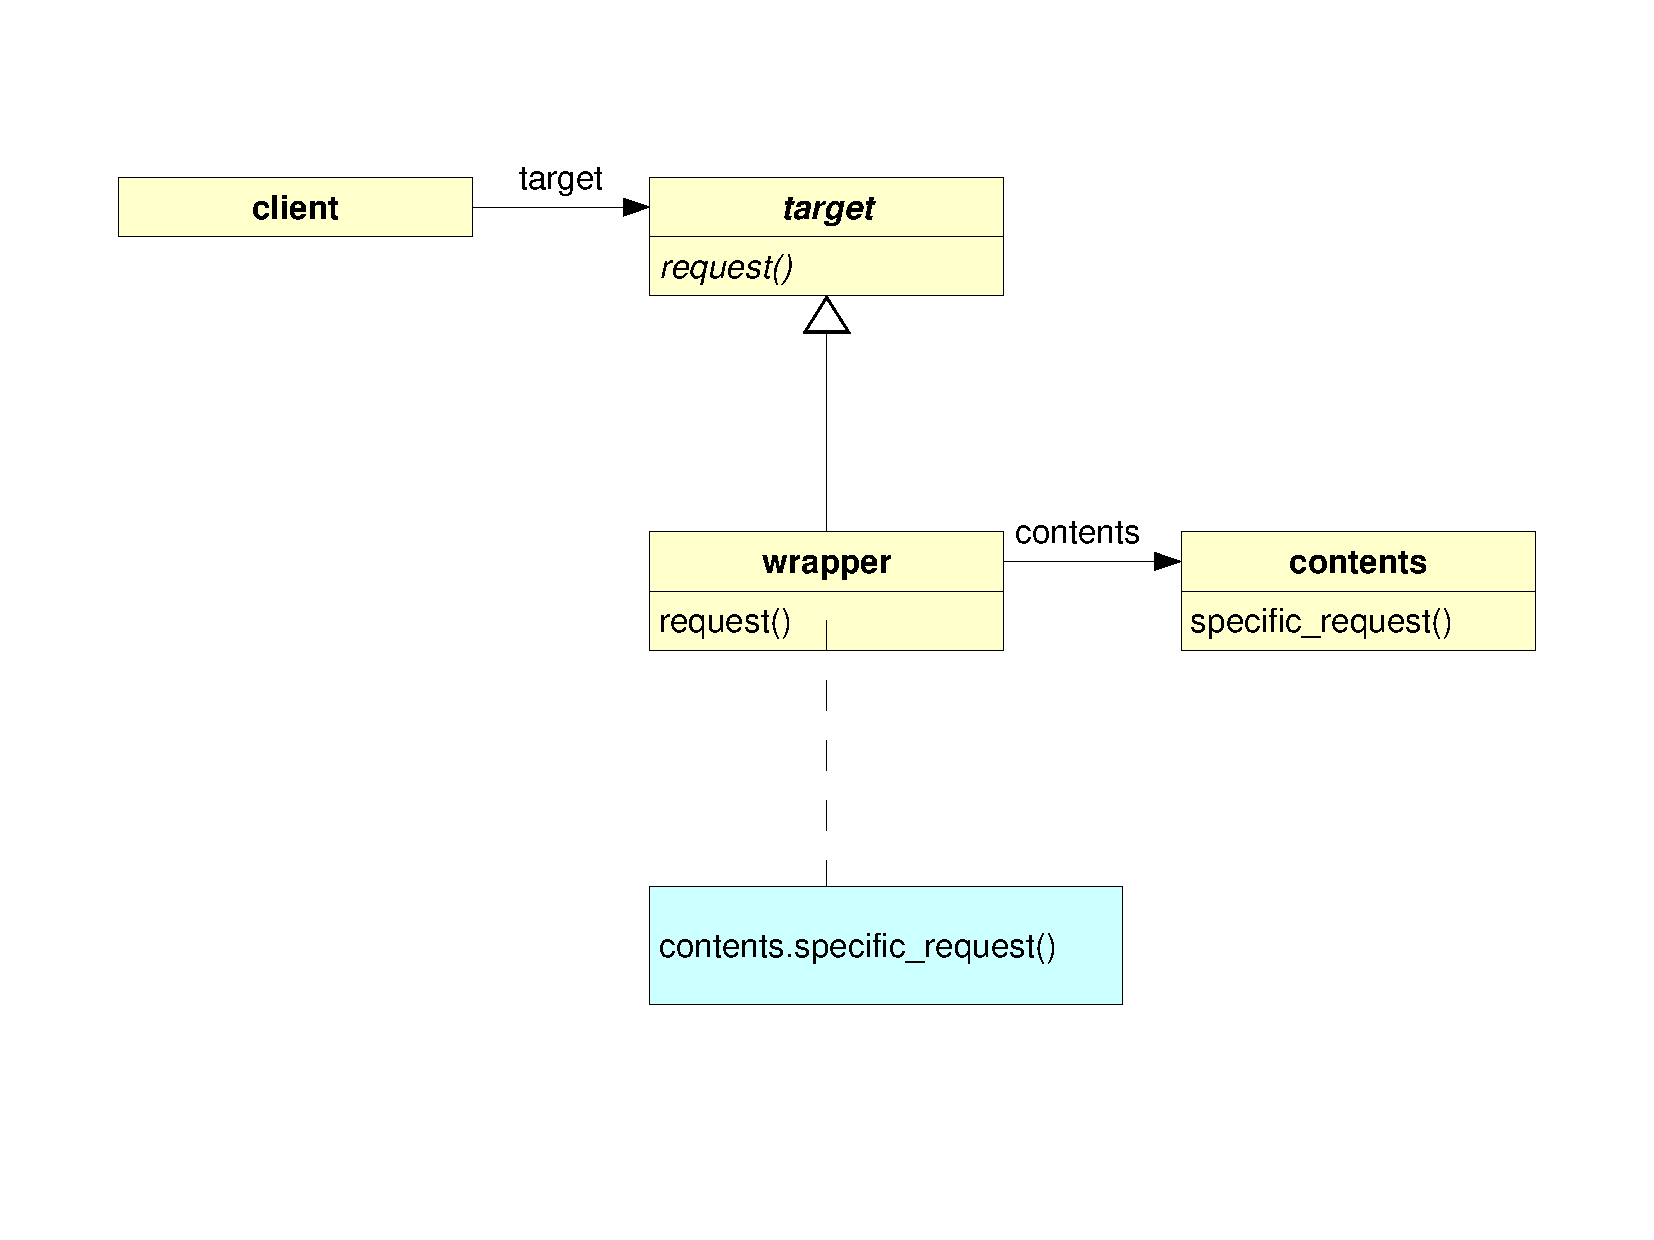
\includegraphics[scale=0.3,angle=-90]{graphic/wrapper.pdf}
        \caption{Wrapper Pattern}
        \label{wrapper_figure}
    \end{center}
\end{figure}

Knowledge templates created in the language described in chapter
\ref{cybernetics_oriented_language_heading} wrap the more fine-granular
templates they consist of.

%
% $RCSfile: whole_part.tex,v $
%
% Copyright (c) 2004. Christian Heller. All rights reserved.
%
% No copying, altering, distribution or any other actions concerning this
% document, except after explicit permission by the author!
% At some later point in time, this document is planned to be put under
% the GNU FDL license. For now, _everything_ is _restricted_ by the author.
%
% http://www.cybop.net
% - Cybernetics Oriented Programming -
%
% http://www.resmedicinae.org
% - Information in Medicine -
%
% @author Christian Heller <christian.heller@tuxtax.de>
%

\paragraph{Whole Part}
\label{whole_part_heading}

Whenever many components form a semantic unit, they can be subsumed by the
\emph{Whole-Part} pattern \cite{buschmann}. It encapsulates single part objects
(figure \ref{wholepart_figure}) and controls their cooperation. Part objects
are not addressable directly.

Almost all software systems contain components or sub systems which could be
organized by help of this pattern. In some way, it is quite similar to the
previously introduced \emph{Wrapper}, only that not just one- but many objects
are wrapped.

\begin{figure}[ht]
    \begin{center}
        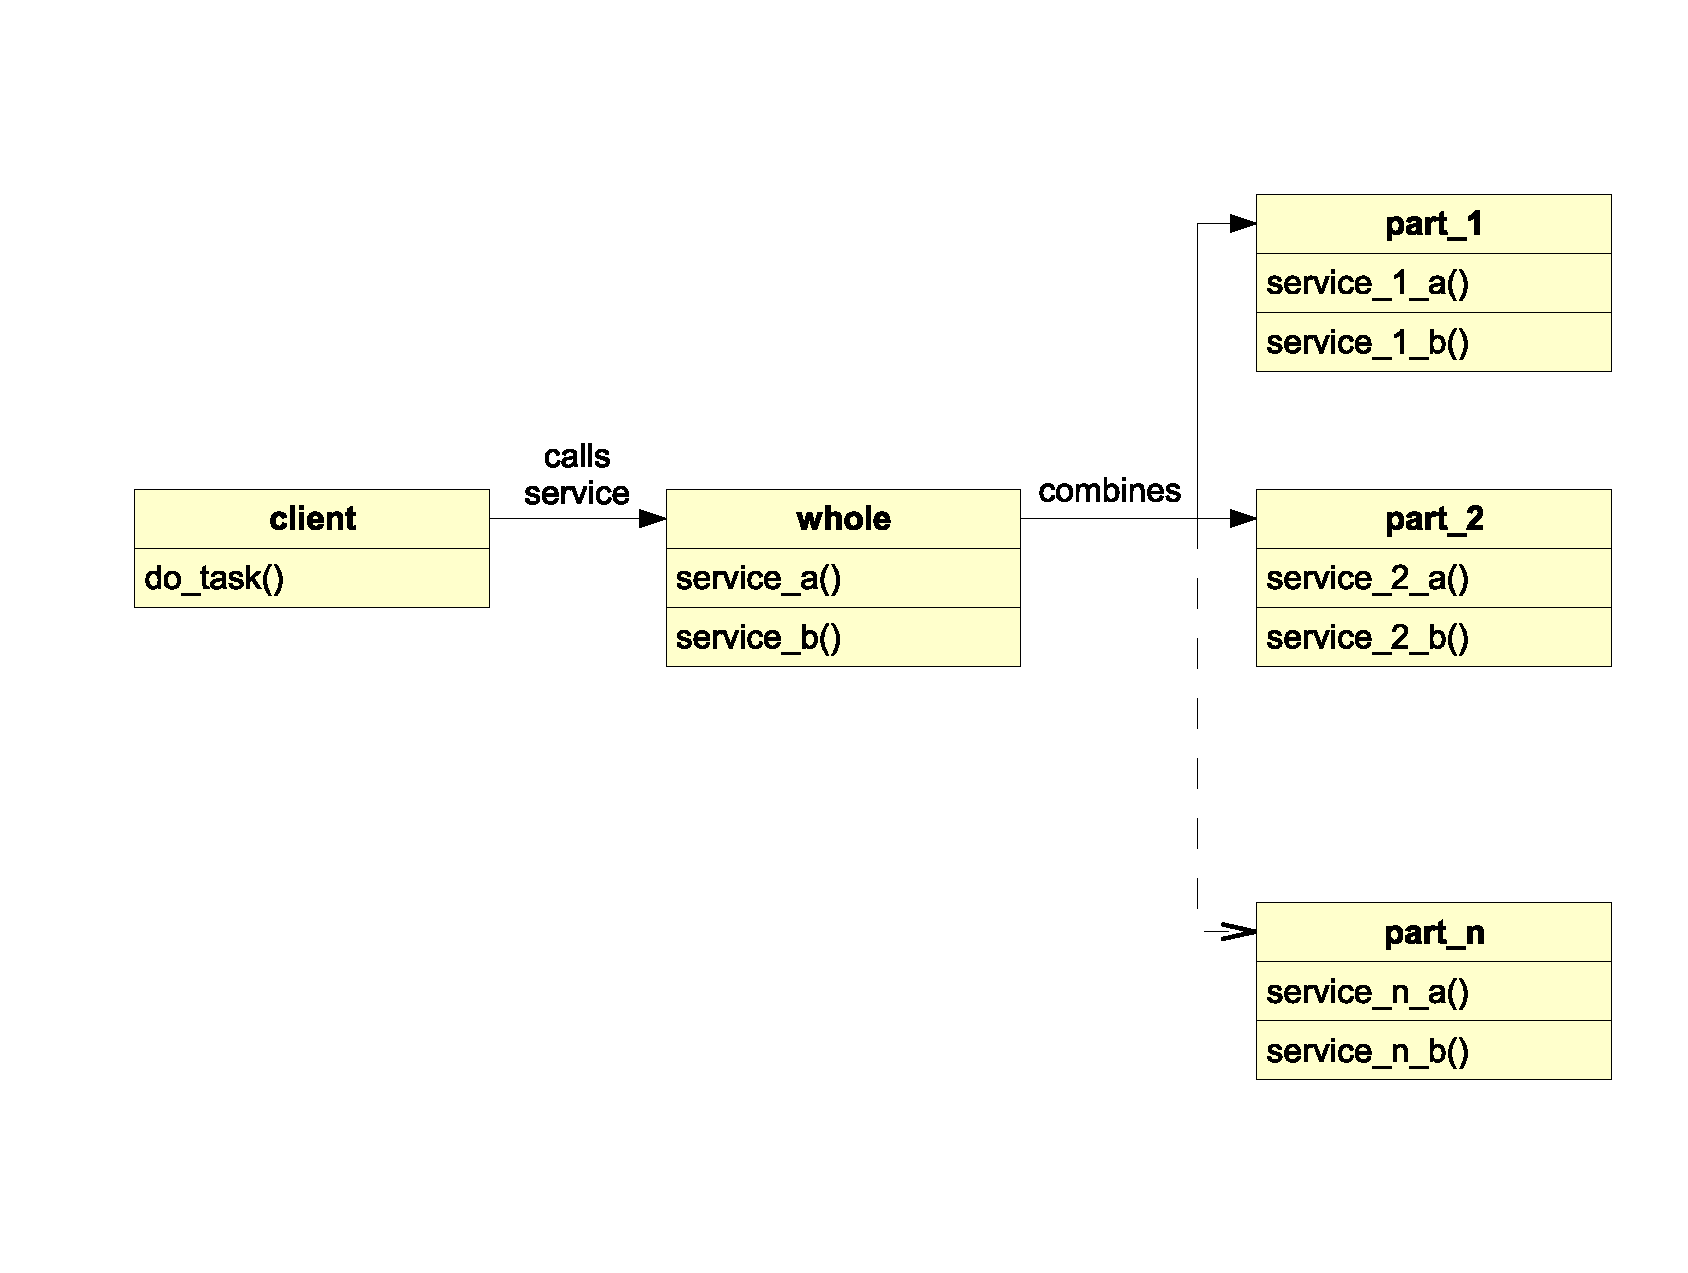
\includegraphics[scale=0.3]{vector/wholepart.eps}
        \caption{Whole-Part Pattern}
        \label{wholepart_figure}
    \end{center}
\end{figure}

%
% $RCSfile: composite.tex,v $
%
% Copyright (c) 2004. Christian Heller. All rights reserved.
%
% No copying, altering, distribution or any other actions concerning this
% document, except after explicit permission by the author!
% At some later point in time, this document is planned to be put under
% the GNU FDL license. For now, _everything_ is _restricted_ by the author.
%
% http://www.cybop.net
% - Cybernetics Oriented Programming -
%
% http://www.resmedicinae.org
% - Information in Medicine -
%
% @author Christian Heller <christian.heller@tuxtax.de>
%

\paragraph{Composite}
\label{composite_heading}

A hierarchical object structure, also called \emph{Directed Acyclical Graph}
(DAG) or \emph{Tree}, can be represented by a combination of classes called
\emph{Composite} pattern \cite{gamma1995}. It describes a \emph{Component} that
may consist of \emph{Children} (figure \ref{composite_figure}), which makes it
comparable to the \emph{Whole-Part} pattern. The difference is that the
\emph{Composite} is a more generalized version, with a dynamically extensible
number of child (part) objects.

The \emph{Composite} is a pattern based on \emph{Recursion}, which is one of
the most commonly used programming techniques at all. The pattern's split into
\emph{Leaf-} and \emph{Composite} sub classes helps distinguish primitive- from
container objects. A composite tree node holds objects of type \emph{Component}.

\begin{figure}[ht]
    \begin{center}
        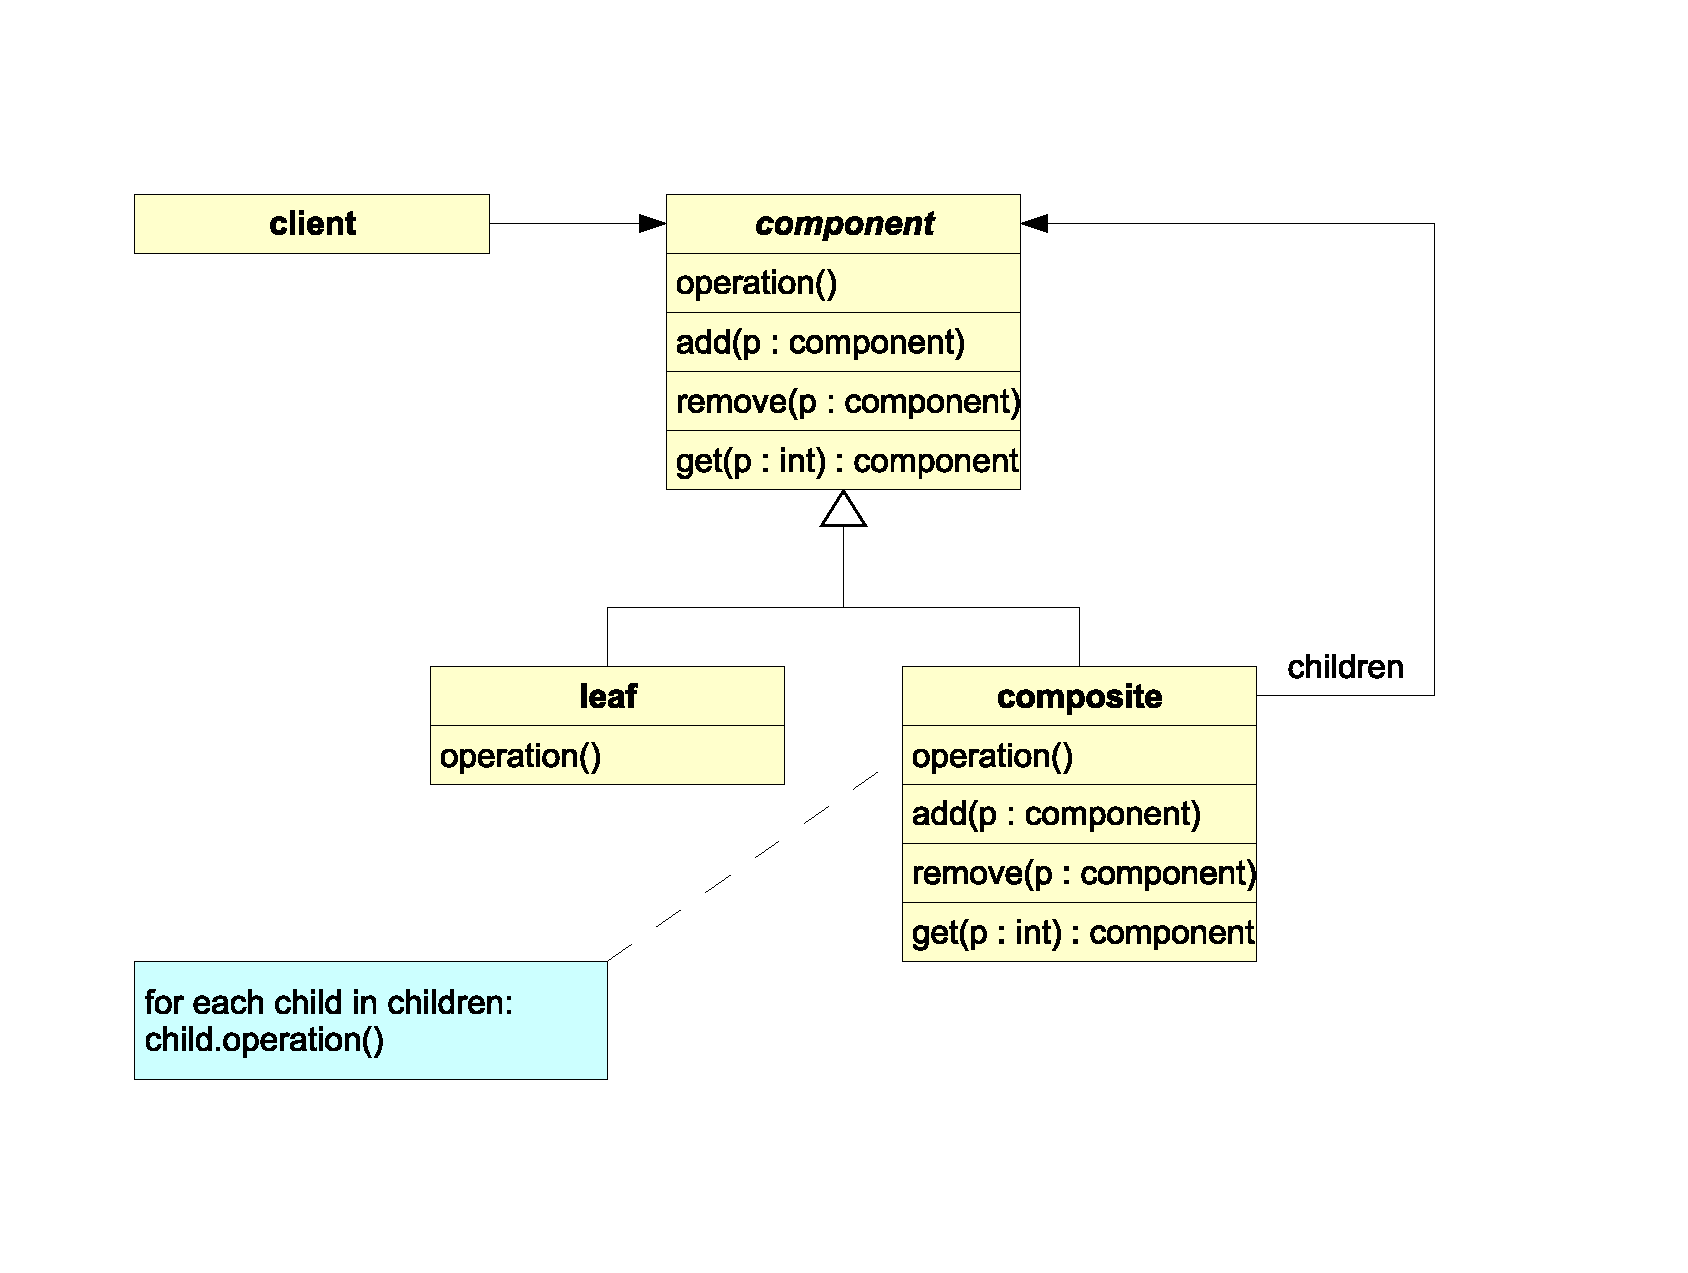
\includegraphics[scale=0.3]{vector/composite.eps}
        \caption{Composite Pattern}
        \label{composite_figure}
    \end{center}
\end{figure}

%
% $RCSfile: chain_of_responsibility.tex,v $
%
% Copyright (c) 2004. Christian Heller. All rights reserved.
%
% No copying, altering, distribution or any other actions concerning this
% document, except after explicit permission by the author!
% At some later point in time, this document is planned to be put under
% the GNU FDL license. For now, _everything_ is _restricted_ by the author.
%
% http://www.cybop.net
% - Cybernetics Oriented Programming -
%
% http://www.resmedicinae.org
% - Information in Medicine -
%
% @author Christian Heller <christian.heller@tuxtax.de>
%

\paragraph{Chain of Responsibility}
\label{chain_of_responsibility_heading}

The \emph{Chain of Responsibility} pattern \cite{gamma1995} is similar to the
\emph{Composite}, in that it represents a recursive structure as well. Objects
destined to solve a task are linked with a corresponding \emph{Successor}
(figure \ref{chain_figure}), such forming a chain. If an object is not able to
solve a task, that task is forwarded to the object's successor, along the chain.

\begin{figure}[ht]
    \begin{center}
        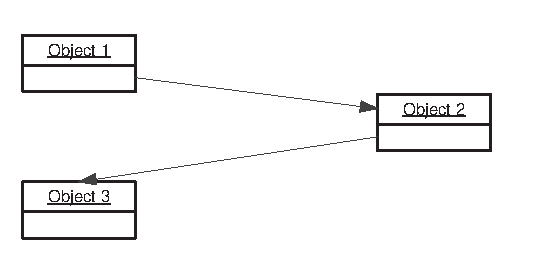
\includegraphics[scale=0.3]{vector/chain.eps}
        \caption{Chain of Responsibility Pattern}
        \label{chain_figure}
    \end{center}
\end{figure}

The pattern found wide application, for example in help systems, in event
handling frameworks or for exception handling. Its \emph{Handler} class is
known under synonyms like \emph{Event Handler}, \emph{Bureaucrat} or
\emph{Responder}.

Frequently, the pattern gets misused by delegating messages not only to children
but also to the parent of objects. The \emph{Hierarhical Model View Controller}
(HMVC) pattern is one example for this. It causes unfavourable bidirectional
dependencies (section \ref{bidirectional_dependency_heading}) and leads to
stronger coupling between the layers of a framework, because parent- and child
objects then reference each other.

%
% $RCSfile: observer.tex,v $
%
% Copyright (c) 2004. Christian Heller. All rights reserved.
%
% No copying, altering, distribution or any other actions concerning this
% document, except after explicit permission by the author!
% At some later point in time, this document is planned to be put under
% the GNU FDL license. For now, _everything_ is _restricted_ by the author.
%
% http://www.cybop.net
% - Cybernetics Oriented Programming -
%
% http://www.resmedicinae.org
% - Information in Medicine -
%
% @author Christian Heller <christian.heller@tuxtax.de>
%

\paragraph{Observer}
\label{observer_heading}

Another pattern that found wide application is the \emph{Observer} \cite{gamma1995},
an often-used synonym for which is \emph{Publisher-Subscriber}. It provides a
notification mechanism for all objects that registered as \emph{Observer} at a
\emph{Subject} in whose state changes they are interested, leading to an automatic
update of all dependent objects (figure \ref{observer_figure}).

\begin{figure}[ht]
    \begin{center}
        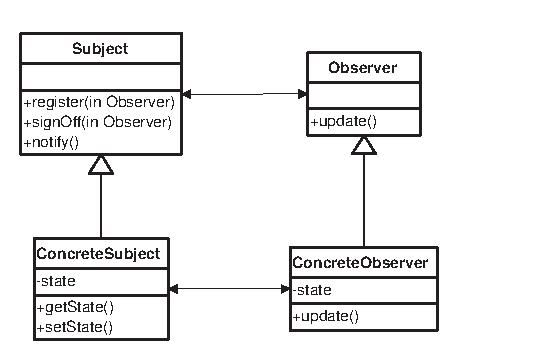
\includegraphics[scale=0.3]{vector/observer.eps}
        \caption{Observer Pattern}
        \label{observer_figure}
    \end{center}
\end{figure}

\begin{figure}[ht]
    \begin{center}
        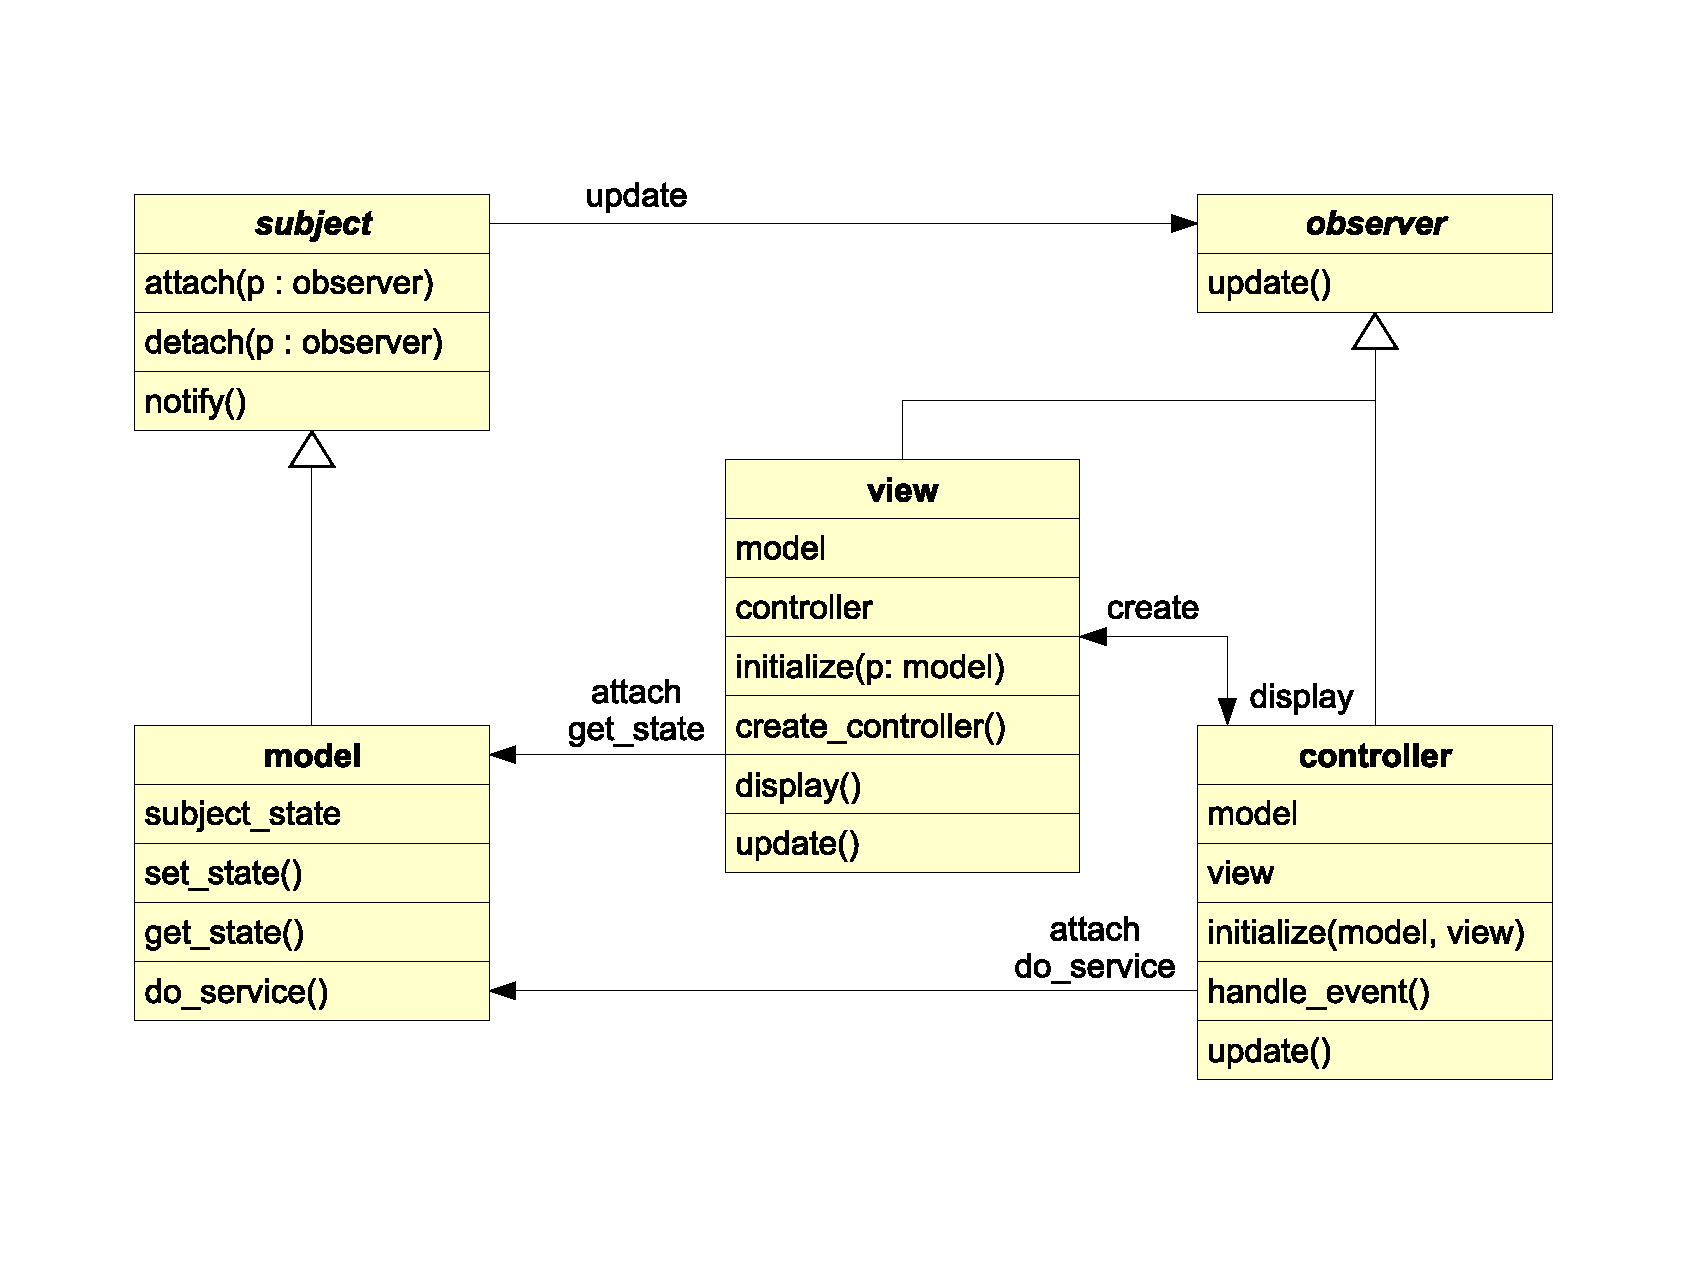
\includegraphics[scale=0.3]{vector/mvcobserver.eps}
        \caption{MVC- using Observer Pattern}
        \label{mvcobserver_figure}
    \end{center}
\end{figure}

Similar notification mechanisms are used for \emph{Callback} event handling in
frameworks, where the framework core calls functionality of its extensions. The
\emph{Model View Controller-} (MVC) uses the \emph{Observer} pattern to let the
model notify its observing views about necessary updates (figure
\ref{mvcobserver_figure}).

A disadvantage of the \emph{Observer} pattern is that it relies on bidirectional
dependencies (section \ref{bidirectional_dependency_heading}), so that circular
references can occur, when a system is not programmed very carefully.

%
% $RCSfile: bidirectional_dependency.tex,v $
%
% Copyright (C) 2002-2008. Christian Heller.
%
% Permission is granted to copy, distribute and/or modify this document
% under the terms of the GNU Free Documentation License, Version 1.1 or
% any later version published by the Free Software Foundation; with no
% Invariant Sections, with no Front-Cover Texts and with no Back-Cover
% Texts. A copy of the license is included in the section entitled
% "GNU Free Documentation License".
%
% http://www.cybop.net
% - Cybernetics Oriented Programming -
%
% http://www.resmedicinae.org
% - Information in Medicine -
%
% Version: $Revision: 1.1 $ $Date: 2008-08-19 20:41:05 $ $Author: christian $
% Authors: Christian Heller <christian.heller@tuxtax.de>
%

\subsubsection{Bidirectional Dependency}
\label{bidirectional_dependency_heading}
\index{Bidirectional Dependency}
\index{Inter-Dependency}
\index{Endless Loop}
\index{Tree}
\index{Directed Acyclic Graph}
\index{DAG}
\index{Oriented Acyclic Graph}
\index{Process Tree}
\index{Object Tree}
\index{Database Data Structure}
\index{File System Structure}
\index{Syntax Tree}
\index{Acyclic Graph}
\index{Circular Reference}

\emph{Bidirectional References} are a nightmare for every software developer.
They cause \emph{Inter-Dependencies} so that changes in one part of a system can
affect multiple other parts which in turn affect the originating part, which may
finally lead to cycles or even endless loops. Also, the actual program flow and
effects of changes to a system become very hard to trace. Therefore, the avoidance
of such dependencies belongs to the core principles of good software design.

A \emph{Tree}, in mathematics, is defined as \textit{Directed Acyclic Graph}
(DAG), also known as \emph{Oriented Acyclic Graph} \cite{nist}. It has a
\emph{Root Node} and \emph{Child Nodes} which can become \emph{Parent Nodes}
when having children themselves; otherwise they are called \emph{Leaves}.
Children of the same node are \emph{Siblings}. \textit{A common constraint is
that no node can have more than one parent}, as \cite{foldoc} writes and
continues: \textit{Moreover, for some applications, it is necessary to consider
a node's children to be an ordered list, instead of merely a set.} A graph is
\emph{acyclic} if every node can be reached via exactly one path, which then
also is the shortest possible.

In computing, trees are used in many forms, for example as \emph{Process Tree}
of an operating system \cite{debian, gnu, linux} or as \emph{Object Tree} of an
object-oriented application. They represent \emph{Data Structures} in databases
or file systems and also the \emph{Syntax Tree} of languages. The violation of
the principle of the \emph{Acyclic Graph} can lead to the same loops, also
called \emph{Circular References}, as mentioned above, which can result in the
crossing of memory limits and is a potential security risk. Therefore, one of
the main aims in the creation of the new concepts introduced in part
\ref{contribution_heading} of this work was the avoidance of bidirectional
relations.

